\documentclass[1p]{elsarticle_modified}
%\bibliographystyle{elsarticle-num}

%\usepackage[colorlinks]{hyperref}
%\usepackage{abbrmath_seonhwa} %\Abb, \Ascr, \Acal ,\Abf, \Afrak
\usepackage{amsfonts}
\usepackage{amssymb}
\usepackage{amsmath}
\usepackage{amsthm}
\usepackage{scalefnt}
\usepackage{amsbsy}
\usepackage{kotex}
\usepackage{caption}
\usepackage{subfig}
\usepackage{color}
\usepackage{graphicx}
\usepackage{xcolor} %% white, black, red, green, blue, cyan, magenta, yellow
\usepackage{float}
\usepackage{setspace}
\usepackage{hyperref}

\usepackage{tikz}
\usetikzlibrary{arrows}

\usepackage{multirow}
\usepackage{array} % fixed length table
\usepackage{hhline}

%%%%%%%%%%%%%%%%%%%%%
\makeatletter
\renewcommand*\env@matrix[1][\arraystretch]{%
	\edef\arraystretch{#1}%
	\hskip -\arraycolsep
	\let\@ifnextchar\new@ifnextchar
	\array{*\c@MaxMatrixCols c}}
\makeatother %https://tex.stackexchange.com/questions/14071/how-can-i-increase-the-line-spacing-in-a-matrix
%%%%%%%%%%%%%%%

\usepackage[normalem]{ulem}

\newcommand{\msout}[1]{\ifmmode\text{\sout{\ensuremath{#1}}}\else\sout{#1}\fi}
%SOURCE: \msout is \stkout macro in https://tex.stackexchange.com/questions/20609/strikeout-in-math-mode

\newcommand{\cancel}[1]{
	\ifmmode
	{\color{red}\msout{#1}}
	\else
	{\color{red}\sout{#1}}
	\fi
}

\newcommand{\add}[1]{
	{\color{blue}\uwave{#1}}
}

\newcommand{\replace}[2]{
	\ifmmode
	{\color{red}\msout{#1}}{\color{blue}\uwave{#2}}
	\else
	{\color{red}\sout{#1}}{\color{blue}\uwave{#2}}
	\fi
}

\newcommand{\Sol}{\mathcal{S}} %segment
\newcommand{\D}{D} %diagram
\newcommand{\A}{\mathcal{A}} %arc


%%%%%%%%%%%%%%%%%%%%%%%%%%%%%5 test

\def\sl{\operatorname{\textup{SL}}(2,\Cbb)}
\def\psl{\operatorname{\textup{PSL}}(2,\Cbb)}
\def\quan{\mkern 1mu \triangleright \mkern 1mu}

\theoremstyle{definition}
\newtheorem{thm}{Theorem}[section]
\newtheorem{prop}[thm]{Proposition}
\newtheorem{lem}[thm]{Lemma}
\newtheorem{ques}[thm]{Question}
\newtheorem{cor}[thm]{Corollary}
\newtheorem{defn}[thm]{Definition}
\newtheorem{exam}[thm]{Example}
\newtheorem{rmk}[thm]{Remark}
\newtheorem{alg}[thm]{Algorithm}

\newcommand{\I}{\sqrt{-1}}
\begin{document}

%\begin{frontmatter}
%
%\title{Boundary parabolic representations of knots up to 8 crossings}
%
%%% Group authors per affiliation:
%\author{Yunhi Cho} 
%\address{Department of Mathematics, University of Seoul, Seoul, Korea}
%\ead{yhcho@uos.ac.kr}
%
%
%\author{Seonhwa Kim} %\fnref{s_kim}}
%\address{Center for Geometry and Physics, Institute for Basic Science, Pohang, 37673, Korea}
%\ead{ryeona17@ibs.re.kr}
%
%\author{Hyuk Kim}
%\address{Department of Mathematical Sciences, Seoul National University, Seoul 08826, Korea}
%\ead{hyukkim@snu.ac.kr}
%
%\author{Seokbeom Yoon}
%\address{Department of Mathematical Sciences, Seoul National University, Seoul, 08826,  Korea}
%\ead{sbyoon15@snu.ac.kr}
%
%\begin{abstract}
%We find all boundary parabolic representation of knots up to 8 crossings.
%
%\end{abstract}
%\begin{keyword}
%    \MSC[2010] 57M25 
%\end{keyword}
%
%\end{frontmatter}

%\linenumbers
%\tableofcontents
%
\newcommand\colored[1]{\textcolor{white}{\rule[-0.35ex]{0.8em}{1.4ex}}\kern-0.8em\color{red} #1}%
%\newcommand\colored[1]{\textcolor{white}{ #1}\kern-2.17ex	\textcolor{white}{ #1}\kern-1.81ex	\textcolor{white}{ #1}\kern-2.15ex\color{red}#1	}

{\Large $\underline{12a_{0658}~(K12a_{0658})}$}

\setlength{\tabcolsep}{10pt}
\renewcommand{\arraystretch}{1.6}
\vspace{1cm}\begin{tabular}{m{100pt}>{\centering\arraybackslash}m{274pt}}
\multirow{5}{120pt}{
	\centering
	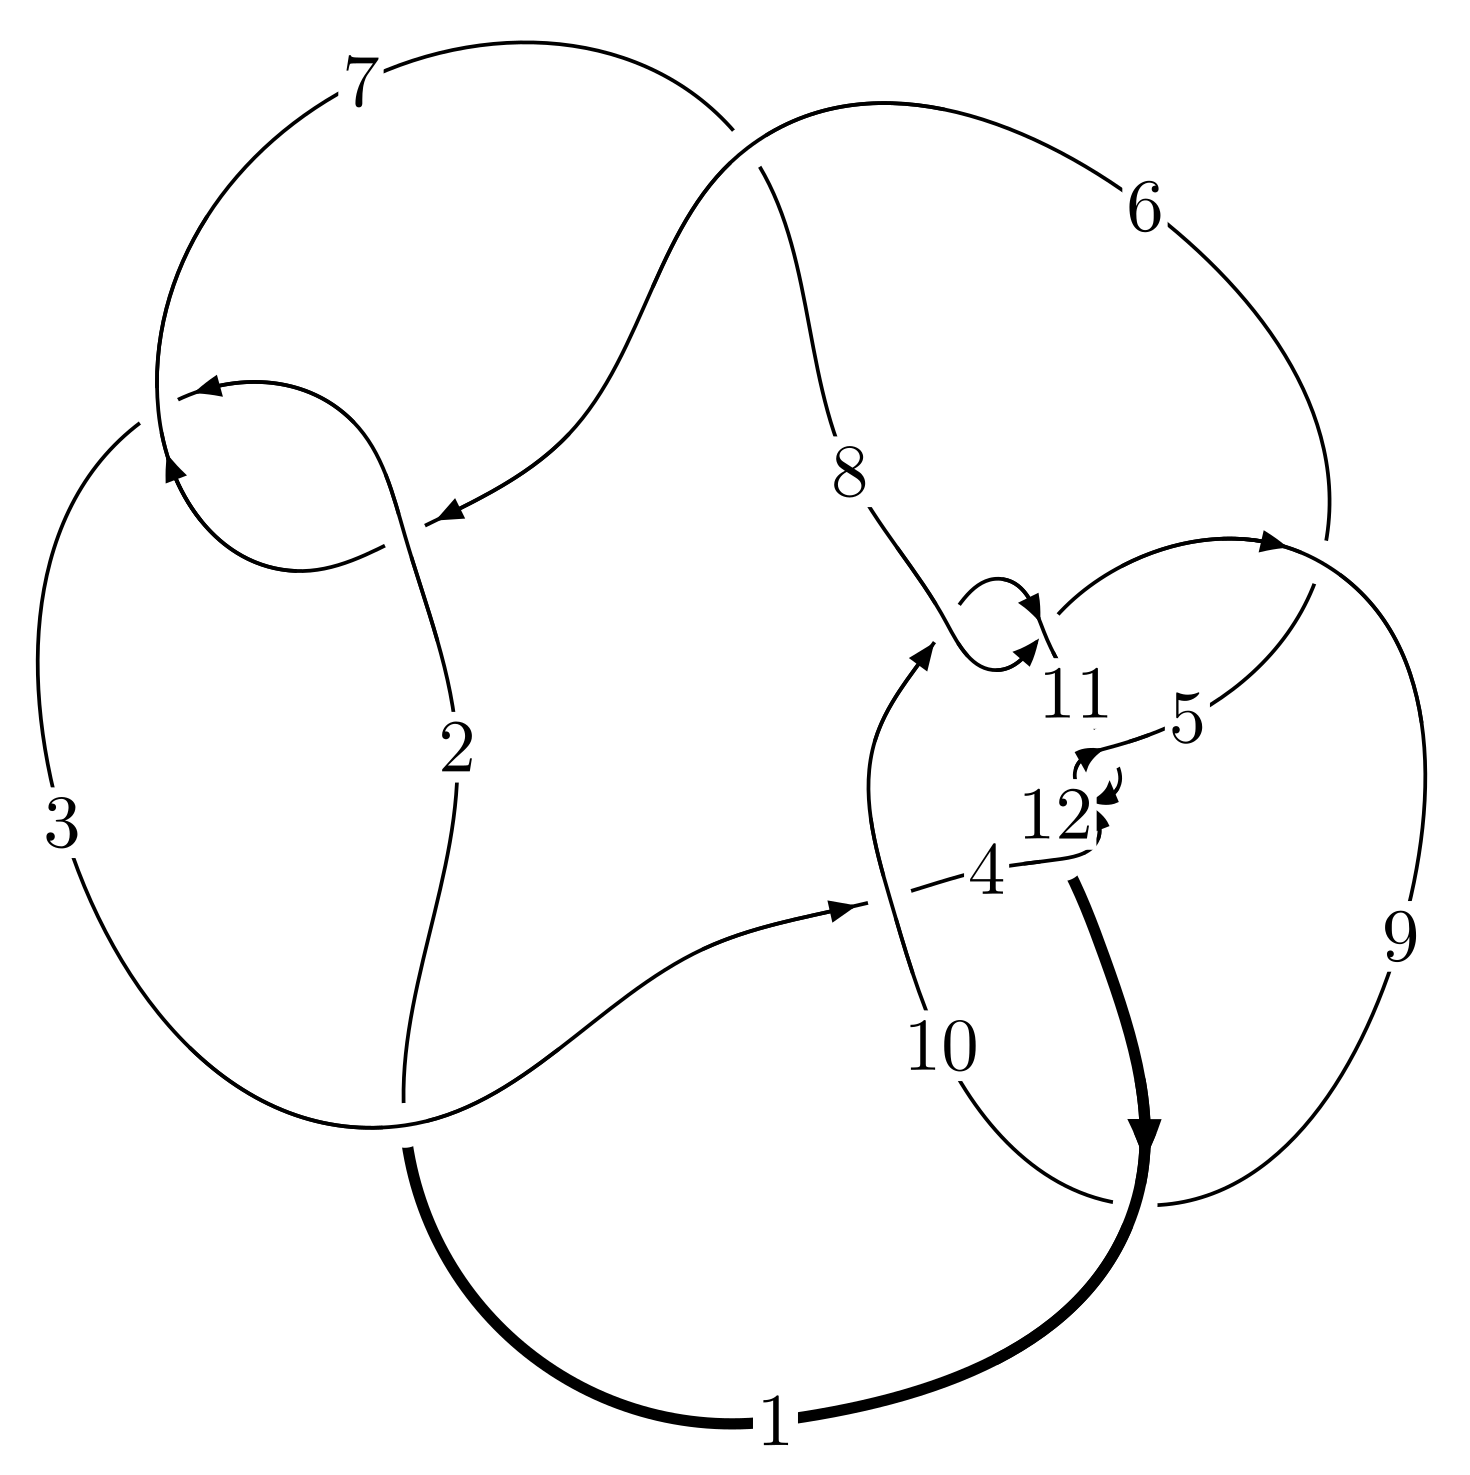
\includegraphics[width=112pt]{../../../GIT/diagram.site/Diagrams/png/1459_12a_0658.png}\\
\ \ \ A knot diagram\footnotemark}&
\allowdisplaybreaks
\textbf{Linearized knot diagam} \\
\cline{2-2}
 &
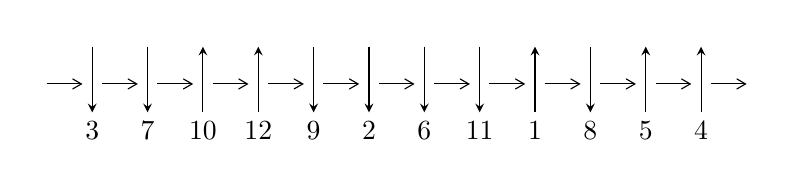
\begin{tikzpicture}[x=20pt, y=17pt]
	% nodes
	\node (C0) at (0, 0) {};
	\node (C1) at (1, 0) {};
	\node (C1U) at (1, +1) {};
	\node (C1D) at (1, -1) {3};

	\node (C2) at (2, 0) {};
	\node (C2U) at (2, +1) {};
	\node (C2D) at (2, -1) {7};

	\node (C3) at (3, 0) {};
	\node (C3U) at (3, +1) {};
	\node (C3D) at (3, -1) {10};

	\node (C4) at (4, 0) {};
	\node (C4U) at (4, +1) {};
	\node (C4D) at (4, -1) {12};

	\node (C5) at (5, 0) {};
	\node (C5U) at (5, +1) {};
	\node (C5D) at (5, -1) {9};

	\node (C6) at (6, 0) {};
	\node (C6U) at (6, +1) {};
	\node (C6D) at (6, -1) {2};

	\node (C7) at (7, 0) {};
	\node (C7U) at (7, +1) {};
	\node (C7D) at (7, -1) {6};

	\node (C8) at (8, 0) {};
	\node (C8U) at (8, +1) {};
	\node (C8D) at (8, -1) {11};

	\node (C9) at (9, 0) {};
	\node (C9U) at (9, +1) {};
	\node (C9D) at (9, -1) {1};

	\node (C10) at (10, 0) {};
	\node (C10U) at (10, +1) {};
	\node (C10D) at (10, -1) {8};

	\node (C11) at (11, 0) {};
	\node (C11U) at (11, +1) {};
	\node (C11D) at (11, -1) {5};

	\node (C12) at (12, 0) {};
	\node (C12U) at (12, +1) {};
	\node (C12D) at (12, -1) {4};
	\node (C13) at (13, 0) {};

	% arrows
	\draw[->,>={angle 60}]
	(C0) edge (C1) (C1) edge (C2) (C2) edge (C3) (C3) edge (C4) (C4) edge (C5) (C5) edge (C6) (C6) edge (C7) (C7) edge (C8) (C8) edge (C9) (C9) edge (C10) (C10) edge (C11) (C11) edge (C12) (C12) edge (C13) ;	\draw[->,>=stealth]
	(C1U) edge (C1D) (C2U) edge (C2D) (C3D) edge (C3U) (C4D) edge (C4U) (C5U) edge (C5D) (C6U) edge (C6D) (C7U) edge (C7D) (C8U) edge (C8D) (C9D) edge (C9U) (C10U) edge (C10D) (C11D) edge (C11U) (C12D) edge (C12U) ;
	\end{tikzpicture} \\
\hhline{~~} \\& 
\textbf{Solving Sequence} \\ \cline{2-2} 
 &
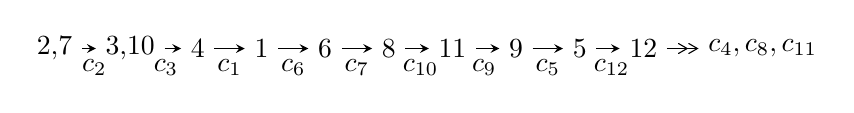
\begin{tikzpicture}[x=23pt, y=7pt]
	% node
	\node (A0) at (-1/8, 0) {2,7};
	\node (A1) at (17/16, 0) {3,10};
	\node (A2) at (17/8, 0) {4};
	\node (A3) at (25/8, 0) {1};
	\node (A4) at (33/8, 0) {6};
	\node (A5) at (41/8, 0) {8};
	\node (A6) at (49/8, 0) {11};
	\node (A7) at (57/8, 0) {9};
	\node (A8) at (65/8, 0) {5};
	\node (A9) at (73/8, 0) {12};
	\node (C1) at (1/2, -1) {$c_{2}$};
	\node (C2) at (13/8, -1) {$c_{3}$};
	\node (C3) at (21/8, -1) {$c_{1}$};
	\node (C4) at (29/8, -1) {$c_{6}$};
	\node (C5) at (37/8, -1) {$c_{7}$};
	\node (C6) at (45/8, -1) {$c_{10}$};
	\node (C7) at (53/8, -1) {$c_{9}$};
	\node (C8) at (61/8, -1) {$c_{5}$};
	\node (C9) at (69/8, -1) {$c_{12}$};
	\node (A10) at (11, 0) {$c_{4},c_{8},c_{11}$};

	% edge
	\draw[->,>=stealth]	
	(A0) edge (A1) (A1) edge (A2) (A2) edge (A3) (A3) edge (A4) (A4) edge (A5) (A5) edge (A6) (A6) edge (A7) (A7) edge (A8) (A8) edge (A9) ;
	\draw[->>,>={angle 60}]	
	(A9) edge (A10);
\end{tikzpicture} \\ 

\end{tabular} \\

\footnotetext{
The image of knot diagram is generated by the software ``\textbf{Draw programme}" developed by Andrew Bartholomew(\url{http://www.layer8.co.uk/maths/draw/index.htm\#Running-draw}), where we modified some parts for our purpose(\url{https://github.com/CATsTAILs/LinksPainter}).
}\phantom \\ \newline 
\centering \textbf{Ideals for irreducible components\footnotemark of $X_{\text{par}}$} 
 
\begin{align*}
I^u_{1}&=\langle 
-2.62898\times10^{65} u^{82}-9.33541\times10^{66} u^{81}+\cdots+9.04370\times10^{67} b+3.29825\times10^{66},\\
\phantom{I^u_{1}}&\phantom{= \langle  }2.10524\times10^{67} u^{82}+1.26169\times10^{67} u^{81}+\cdots+9.04370\times10^{67} a+5.17635\times10^{66},\;u^{83}+u^{82}+\cdots-3 u^2-1\rangle \\
\\
\end{align*}
\raggedright * 1 irreducible components of $\dim_{\mathbb{C}}=0$, with total 83 representations.\\
\footnotetext{All coefficients of polynomials are rational numbers. But the coefficients are sometimes approximated in decimal forms when there is not enough margin.}
\newpage
\renewcommand{\arraystretch}{1}
\centering \section*{I. $I^u_{1}= \langle -2.63\times10^{65} u^{82}-9.34\times10^{66} u^{81}+\cdots+9.04\times10^{67} b+3.30\times10^{66},\;2.11\times10^{67} u^{82}+1.26\times10^{67} u^{81}+\cdots+9.04\times10^{67} a+5.18\times10^{66},\;u^{83}+u^{82}+\cdots-3 u^2-1 \rangle$}
\flushleft \textbf{(i) Arc colorings}\\
\begin{tabular}{m{7pt} m{180pt} m{7pt} m{180pt} }
\flushright $a_{2}=$&$\begin{pmatrix}1\\0\end{pmatrix}$ \\
\flushright $a_{7}=$&$\begin{pmatrix}0\\u\end{pmatrix}$ \\
\flushright $a_{3}=$&$\begin{pmatrix}1\\u^2\end{pmatrix}$ \\
\flushright $a_{10}=$&$\begin{pmatrix}-0.232785 u^{82}-0.139510 u^{81}+\cdots+1.16873 u-0.0572371\\0.00290698 u^{82}+0.103226 u^{81}+\cdots+2.00815 u-0.0364701\end{pmatrix}$ \\
\flushright $a_{4}=$&$\begin{pmatrix}6.38689 u^{82}+8.65090 u^{81}+\cdots+6.46944 u+9.73885\\0.0601500 u^{82}-4.03734 u^{81}+\cdots+6.62282 u+6.42267\end{pmatrix}$ \\
\flushright $a_{1}=$&$\begin{pmatrix}- u^2+1\\- u^4\end{pmatrix}$ \\
\flushright $a_{6}=$&$\begin{pmatrix}u\\u\end{pmatrix}$ \\
\flushright $a_{8}=$&$\begin{pmatrix}- u^3\\- u^3+u\end{pmatrix}$ \\
\flushright $a_{11}=$&$\begin{pmatrix}-0.162336 u^{82}-0.0965383 u^{81}+\cdots+1.25096 u-0.0980678\\-0.00887391 u^{82}+0.104798 u^{81}+\cdots+0.973680 u+0.0160412\end{pmatrix}$ \\
\flushright $a_{9}=$&$\begin{pmatrix}-0.237869 u^{82}-0.170081 u^{81}+\cdots-0.811372 u+0.00168075\\0.0182886 u^{82}+0.0928221 u^{81}+\cdots+1.99990 u-0.0425818\end{pmatrix}$ \\
\flushright $a_{5}=$&$\begin{pmatrix}-6.26650 u^{82}-6.25201 u^{81}+\cdots+4.47085 u-6.68810\\-2.39740 u^{82}+4.01692 u^{81}+\cdots-7.66722 u-6.36765\end{pmatrix}$ \\
\flushright $a_{12}=$&$\begin{pmatrix}6.70384 u^{82}+19.4884 u^{81}+\cdots-5.38905 u+1.94050\\12.8932 u^{82}+25.5557 u^{81}+\cdots+1.05907 u+6.64542\end{pmatrix}$\\&\end{tabular}
\flushleft \textbf{(ii) Obstruction class $= -1$}\\~\\
\flushleft \textbf{(iii) Cusp Shapes $= 6.54849 u^{82}+10.1599 u^{81}+\cdots-0.291458 u+0.179307$}\\~\\
\newpage\renewcommand{\arraystretch}{1}
\flushleft \textbf{(iv) u-Polynomials at the component}\newline \\
\begin{tabular}{m{50pt}|m{274pt}}
Crossings & \hspace{64pt}u-Polynomials at each crossing \\
\hline $$\begin{aligned}c_{1},c_{7}\end{aligned}$$&$\begin{aligned}
&u^{83}+25 u^{82}+\cdots-6 u+1
\end{aligned}$\\
\hline $$\begin{aligned}c_{2},c_{6}\end{aligned}$$&$\begin{aligned}
&u^{83}- u^{82}+\cdots+3 u^2+1
\end{aligned}$\\
\hline $$\begin{aligned}c_{3}\end{aligned}$$&$\begin{aligned}
&u^{83}-63 u^{82}+\cdots+2026 u-173
\end{aligned}$\\
\hline $$\begin{aligned}c_{4},c_{11},c_{12}\end{aligned}$$&$\begin{aligned}
&u^{83}+3 u^{82}+\cdots-2 u-1
\end{aligned}$\\
\hline $$\begin{aligned}c_{5}\end{aligned}$$&$\begin{aligned}
&u^{83}+57 u^{82}+\cdots+4370580 u-516739
\end{aligned}$\\
\hline $$\begin{aligned}c_{8},c_{10}\end{aligned}$$&$\begin{aligned}
&u^{83}- u^{82}+\cdots+62 u+1
\end{aligned}$\\
\hline $$\begin{aligned}c_{9}\end{aligned}$$&$\begin{aligned}
&u^{83}-7 u^{82}+\cdots+8 u-1
\end{aligned}$\\
\hline
\end{tabular}\\~\\
\newpage\renewcommand{\arraystretch}{1}
\flushleft \textbf{(v) Riley Polynomials at the component}\newline \\
\begin{tabular}{m{50pt}|m{274pt}}
Crossings & \hspace{64pt}Riley Polynomials at each crossing \\
\hline $$\begin{aligned}c_{1},c_{7}\end{aligned}$$&$\begin{aligned}
&y^{83}+67 y^{82}+\cdots-278 y-1
\end{aligned}$\\
\hline $$\begin{aligned}c_{2},c_{6}\end{aligned}$$&$\begin{aligned}
&y^{83}-25 y^{82}+\cdots-6 y-1
\end{aligned}$\\
\hline $$\begin{aligned}c_{3}\end{aligned}$$&$\begin{aligned}
&y^{83}-1525 y^{82}+\cdots-812330 y-29929
\end{aligned}$\\
\hline $$\begin{aligned}c_{4},c_{11},c_{12}\end{aligned}$$&$\begin{aligned}
&y^{83}+87 y^{82}+\cdots-6 y-1
\end{aligned}$\\
\hline $$\begin{aligned}c_{5}\end{aligned}$$&$\begin{aligned}
&y^{83}-1549 y^{82}+\cdots-1262101601146 y-267019194121
\end{aligned}$\\
\hline $$\begin{aligned}c_{8},c_{10}\end{aligned}$$&$\begin{aligned}
&y^{83}-57 y^{82}+\cdots+1394 y-1
\end{aligned}$\\
\hline $$\begin{aligned}c_{9}\end{aligned}$$&$\begin{aligned}
&y^{83}+3 y^{82}+\cdots-254 y-1
\end{aligned}$\\
\hline
\end{tabular}\\~\\
\newpage\flushleft \textbf{(vi) Complex Volumes and Cusp Shapes}
$$\begin{array}{c|c|c}  
\text{Solutions to }I^u_{1}& \I (\text{vol} + \sqrt{-1}CS) & \text{Cusp shape}\\
 \hline 
\begin{aligned}
u &= -0.755268 + 0.689868 I \\
a &= \phantom{-}1.39106 - 0.73110 I \\
b &= -0.85372 - 1.59878 I\end{aligned}
 & -6.36702 - 1.67327 I & \phantom{-0.000000 } 0 \\ \hline\begin{aligned}
u &= -0.755268 - 0.689868 I \\
a &= \phantom{-}1.39106 + 0.73110 I \\
b &= -0.85372 + 1.59878 I\end{aligned}
 & -6.36702 + 1.67327 I & \phantom{-0.000000 } 0 \\ \hline\begin{aligned}
u &= \phantom{-}0.955926 + 0.196493 I \\
a &= -0.22750 - 2.08453 I \\
b &= -0.156061 - 1.022080 I\end{aligned}
 & -7.37611 - 5.46942 I & \phantom{-0.000000 } 0 \\ \hline\begin{aligned}
u &= \phantom{-}0.955926 - 0.196493 I \\
a &= -0.22750 + 2.08453 I \\
b &= -0.156061 + 1.022080 I\end{aligned}
 & -7.37611 + 5.46942 I & \phantom{-0.000000 } 0 \\ \hline\begin{aligned}
u &= \phantom{-}0.956828 + 0.058122 I \\
a &= -2.00868 - 1.22339 I \\
b &= -1.63195 - 0.51030 I\end{aligned}
 & -11.35230 - 2.20989 I & -15.1094 + 3.1648 I \\ \hline\begin{aligned}
u &= \phantom{-}0.956828 - 0.058122 I \\
a &= -2.00868 + 1.22339 I \\
b &= -1.63195 + 0.51030 I\end{aligned}
 & -11.35230 + 2.20989 I & -15.1094 - 3.1648 I \\ \hline\begin{aligned}
u &= \phantom{-}0.687528 + 0.643247 I \\
a &= \phantom{-}0.926393 - 0.698284 I \\
b &= \phantom{-}1.132660 + 0.246219 I\end{aligned}
 & -1.83104 - 2.29304 I & \phantom{-0.000000 } 0 \\ \hline\begin{aligned}
u &= \phantom{-}0.687528 - 0.643247 I \\
a &= \phantom{-}0.926393 + 0.698284 I \\
b &= \phantom{-}1.132660 - 0.246219 I\end{aligned}
 & -1.83104 + 2.29304 I & \phantom{-0.000000 } 0 \\ \hline\begin{aligned}
u &= \phantom{-}0.792394 + 0.712520 I \\
a &= -1.54071 - 0.89895 I \\
b &= \phantom{-}0.35084 - 1.82511 I\end{aligned}
 & \phantom{-}0.299391 + 0.398880 I & \phantom{-0.000000 } 0 \\ \hline\begin{aligned}
u &= \phantom{-}0.792394 - 0.712520 I \\
a &= -1.54071 + 0.89895 I \\
b &= \phantom{-}0.35084 + 1.82511 I\end{aligned}
 & \phantom{-}0.299391 - 0.398880 I & \phantom{-0.000000 } 0\\
 \hline 
 \end{array}$$\newpage$$\begin{array}{c|c|c}  
\text{Solutions to }I^u_{1}& \I (\text{vol} + \sqrt{-1}CS) & \text{Cusp shape}\\
 \hline 
\begin{aligned}
u &= -0.904497 + 0.220913 I \\
a &= \phantom{-}0.17765 - 1.52628 I \\
b &= -0.029075 - 0.629089 I\end{aligned}
 & -1.20857 + 3.31837 I & -4.51564 - 9.28081 I \\ \hline\begin{aligned}
u &= -0.904497 - 0.220913 I \\
a &= \phantom{-}0.17765 + 1.52628 I \\
b &= -0.029075 + 0.629089 I\end{aligned}
 & -1.20857 - 3.31837 I & -4.51564 + 9.28081 I \\ \hline\begin{aligned}
u &= -0.910106 + 0.059437 I \\
a &= \phantom{-}1.27235 - 0.99553 I \\
b &= \phantom{-}1.354240 - 0.173525 I\end{aligned}
 & -4.57106 + 1.49550 I & -13.9394 - 4.6490 I \\ \hline\begin{aligned}
u &= -0.910106 - 0.059437 I \\
a &= \phantom{-}1.27235 + 0.99553 I \\
b &= \phantom{-}1.354240 + 0.173525 I\end{aligned}
 & -4.57106 - 1.49550 I & -13.9394 + 4.6490 I \\ \hline\begin{aligned}
u &= -0.887492 + 0.636493 I \\
a &= \phantom{-}0.683971 - 0.824958 I \\
b &= -0.671063 + 0.175785 I\end{aligned}
 & -8.30238 + 2.46513 I & \phantom{-0.000000 } 0 \\ \hline\begin{aligned}
u &= -0.887492 - 0.636493 I \\
a &= \phantom{-}0.683971 + 0.824958 I \\
b &= -0.671063 - 0.175785 I\end{aligned}
 & -8.30238 - 2.46513 I & \phantom{-0.000000 } 0 \\ \hline\begin{aligned}
u &= \phantom{-}0.875962 + 0.673460 I \\
a &= -0.806933 + 0.072405 I \\
b &= -0.225907 + 0.407373 I\end{aligned}
 & -1.37629 - 2.60149 I & \phantom{-0.000000 } 0 \\ \hline\begin{aligned}
u &= \phantom{-}0.875962 - 0.673460 I \\
a &= -0.806933 - 0.072405 I \\
b &= -0.225907 - 0.407373 I\end{aligned}
 & -1.37629 + 2.60149 I & \phantom{-0.000000 } 0 \\ \hline\begin{aligned}
u &= -0.661827 + 0.885032 I \\
a &= -0.964523 + 0.509781 I \\
b &= \phantom{-}0.022493 + 1.391210 I\end{aligned}
 & \phantom{-}2.87924 - 1.90637 I & \phantom{-0.000000 } 0 \\ \hline\begin{aligned}
u &= -0.661827 - 0.885032 I \\
a &= -0.964523 - 0.509781 I \\
b &= \phantom{-}0.022493 - 1.391210 I\end{aligned}
 & \phantom{-}2.87924 + 1.90637 I & \phantom{-0.000000 } 0\\
 \hline 
 \end{array}$$\newpage$$\begin{array}{c|c|c}  
\text{Solutions to }I^u_{1}& \I (\text{vol} + \sqrt{-1}CS) & \text{Cusp shape}\\
 \hline 
\begin{aligned}
u &= -0.835653 + 0.725148 I \\
a &= \phantom{-}2.60784 - 1.24490 I \\
b &= \phantom{-}0.75247 - 2.72826 I\end{aligned}
 & \phantom{-}1.27283 + 1.90992 I & \phantom{-0.000000 } 0 \\ \hline\begin{aligned}
u &= -0.835653 - 0.725148 I \\
a &= \phantom{-}2.60784 + 1.24490 I \\
b &= \phantom{-}0.75247 + 2.72826 I\end{aligned}
 & \phantom{-}1.27283 - 1.90992 I & \phantom{-0.000000 } 0 \\ \hline\begin{aligned}
u &= -0.759362 + 0.807841 I \\
a &= \phantom{-}1.143780 - 0.638739 I \\
b &= \phantom{-}0.10158 - 2.38329 I\end{aligned}
 & -0.92315 - 4.32848 I & \phantom{-0.000000 } 0 \\ \hline\begin{aligned}
u &= -0.759362 - 0.807841 I \\
a &= \phantom{-}1.143780 + 0.638739 I \\
b &= \phantom{-}0.10158 + 2.38329 I\end{aligned}
 & -0.92315 + 4.32848 I & \phantom{-0.000000 } 0 \\ \hline\begin{aligned}
u &= \phantom{-}0.146295 + 0.862891 I \\
a &= \phantom{-}0.502919 - 0.599119 I \\
b &= \phantom{-}0.318232 + 0.048877 I\end{aligned}
 & -1.16072 - 3.54724 I & -1.48488 + 10.43399 I \\ \hline\begin{aligned}
u &= \phantom{-}0.146295 - 0.862891 I \\
a &= \phantom{-}0.502919 + 0.599119 I \\
b &= \phantom{-}0.318232 - 0.048877 I\end{aligned}
 & -1.16072 + 3.54724 I & -1.48488 - 10.43399 I \\ \hline\begin{aligned}
u &= \phantom{-}0.781550 + 0.815567 I \\
a &= -0.931448 - 0.568907 I \\
b &= -0.16327 - 1.94279 I\end{aligned}
 & \phantom{-}5.31516 + 1.68799 I & \phantom{-0.000000 } 0 \\ \hline\begin{aligned}
u &= \phantom{-}0.781550 - 0.815567 I \\
a &= -0.931448 + 0.568907 I \\
b &= -0.16327 + 1.94279 I\end{aligned}
 & \phantom{-}5.31516 - 1.68799 I & \phantom{-0.000000 } 0 \\ \hline\begin{aligned}
u &= \phantom{-}0.700806 + 0.886878 I \\
a &= \phantom{-}1.07343 + 0.97806 I \\
b &= -0.40330 + 1.95285 I\end{aligned}
 & \phantom{-}2.12600 + 7.17684 I & \phantom{-0.000000 } 0 \\ \hline\begin{aligned}
u &= \phantom{-}0.700806 - 0.886878 I \\
a &= \phantom{-}1.07343 - 0.97806 I \\
b &= -0.40330 - 1.95285 I\end{aligned}
 & \phantom{-}2.12600 - 7.17684 I & \phantom{-0.000000 } 0\\
 \hline 
 \end{array}$$\newpage$$\begin{array}{c|c|c}  
\text{Solutions to }I^u_{1}& \I (\text{vol} + \sqrt{-1}CS) & \text{Cusp shape}\\
 \hline 
\begin{aligned}
u &= -0.835930 + 0.195360 I \\
a &= \phantom{-}1.46241 - 0.35911 I \\
b &= -0.380020 + 0.200495 I\end{aligned}
 & -6.95212 - 0.78250 I & -9.57348 - 2.76568 I \\ \hline\begin{aligned}
u &= -0.835930 - 0.195360 I \\
a &= \phantom{-}1.46241 + 0.35911 I \\
b &= -0.380020 - 0.200495 I\end{aligned}
 & -6.95212 + 0.78250 I & -9.57348 + 2.76568 I \\ \hline\begin{aligned}
u &= -0.715123 + 0.890294 I \\
a &= -1.04148 + 1.30724 I \\
b &= \phantom{-}0.78013 + 2.24858 I\end{aligned}
 & -5.16586 - 10.89950 I & \phantom{-0.000000 } 0 \\ \hline\begin{aligned}
u &= -0.715123 - 0.890294 I \\
a &= -1.04148 - 1.30724 I \\
b &= \phantom{-}0.78013 - 2.24858 I\end{aligned}
 & -5.16586 + 10.89950 I & \phantom{-0.000000 } 0 \\ \hline\begin{aligned}
u &= \phantom{-}1.115590 + 0.254027 I \\
a &= \phantom{-}0.455845 + 0.985086 I \\
b &= \phantom{-}0.752013 + 0.094668 I\end{aligned}
 & -12.8738 - 10.9955 I & \phantom{-0.000000 } 0 \\ \hline\begin{aligned}
u &= \phantom{-}1.115590 - 0.254027 I \\
a &= \phantom{-}0.455845 - 0.985086 I \\
b &= \phantom{-}0.752013 - 0.094668 I\end{aligned}
 & -12.8738 + 10.9955 I & \phantom{-0.000000 } 0 \\ \hline\begin{aligned}
u &= \phantom{-}0.873414 + 0.747229 I \\
a &= -18.3435 - 31.1898 I \\
b &= \phantom{-}7.4711 - 40.6923 I\end{aligned}
 & -3.55022 - 2.83360 I & \phantom{-0.000000 } 0 \\ \hline\begin{aligned}
u &= \phantom{-}0.873414 - 0.747229 I \\
a &= -18.3435 + 31.1898 I \\
b &= \phantom{-}7.4711 + 40.6923 I\end{aligned}
 & -3.55022 + 2.83360 I & \phantom{-0.000000 } 0 \\ \hline\begin{aligned}
u &= -0.904821 + 0.717976 I \\
a &= -1.83061 + 1.76546 I \\
b &= -0.38042 + 3.47812 I\end{aligned}
 & \phantom{-}1.05940 + 3.60208 I & \phantom{-0.000000 } 0 \\ \hline\begin{aligned}
u &= -0.904821 - 0.717976 I \\
a &= -1.83061 - 1.76546 I \\
b &= -0.38042 - 3.47812 I\end{aligned}
 & \phantom{-}1.05940 - 3.60208 I & \phantom{-0.000000 } 0\\
 \hline 
 \end{array}$$\newpage$$\begin{array}{c|c|c}  
\text{Solutions to }I^u_{1}& \I (\text{vol} + \sqrt{-1}CS) & \text{Cusp shape}\\
 \hline 
\begin{aligned}
u &= \phantom{-}0.893817 + 0.740208 I \\
a &= \phantom{-}1.00833 - 1.34709 I \\
b &= \phantom{-}1.86663 - 0.41544 I\end{aligned}
 & -1.93473 - 2.81075 I & \phantom{-0.000000 } 0 \\ \hline\begin{aligned}
u &= \phantom{-}0.893817 - 0.740208 I \\
a &= \phantom{-}1.00833 + 1.34709 I \\
b &= \phantom{-}1.86663 + 0.41544 I\end{aligned}
 & -1.93473 + 2.81075 I & \phantom{-0.000000 } 0 \\ \hline\begin{aligned}
u &= -1.137010 + 0.238482 I \\
a &= -0.311301 + 0.663025 I \\
b &= -0.670008 + 0.007941 I\end{aligned}
 & -5.49259 + 7.04236 I & \phantom{-0.000000 } 0 \\ \hline\begin{aligned}
u &= -1.137010 - 0.238482 I \\
a &= -0.311301 - 0.663025 I \\
b &= -0.670008 - 0.007941 I\end{aligned}
 & -5.49259 - 7.04236 I & \phantom{-0.000000 } 0 \\ \hline\begin{aligned}
u &= -0.816117 + 0.827408 I \\
a &= \phantom{-}0.526716 - 0.470929 I \\
b &= \phantom{-}0.079622 - 1.300680 I\end{aligned}
 & \phantom{-}4.85499 + 2.01628 I & \phantom{-0.000000 } 0 \\ \hline\begin{aligned}
u &= -0.816117 - 0.827408 I \\
a &= \phantom{-}0.526716 + 0.470929 I \\
b &= \phantom{-}0.079622 + 1.300680 I\end{aligned}
 & \phantom{-}4.85499 - 2.01628 I & \phantom{-0.000000 } 0 \\ \hline\begin{aligned}
u &= \phantom{-}0.830299\phantom{ +0.000000I} \\
a &= \phantom{-}0.547895\phantom{ +0.000000I} \\
b &= -2.11831\phantom{ +0.000000I}\end{aligned}
 & -3.06730\phantom{ +0.000000I} & \phantom{-}24.2670\phantom{ +0.000000I} \\ \hline\begin{aligned}
u &= \phantom{-}0.933394 + 0.705292 I \\
a &= \phantom{-}1.70582 + 0.14953 I \\
b &= \phantom{-}1.11542 + 2.14592 I\end{aligned}
 & -0.13209 - 5.84066 I & \phantom{-0.000000 } 0 \\ \hline\begin{aligned}
u &= \phantom{-}0.933394 - 0.705292 I \\
a &= \phantom{-}1.70582 - 0.14953 I \\
b &= \phantom{-}1.11542 - 2.14592 I\end{aligned}
 & -0.13209 + 5.84066 I & \phantom{-0.000000 } 0 \\ \hline\begin{aligned}
u &= -1.126850 + 0.320440 I \\
a &= -0.982231 - 0.060209 I \\
b &= -0.846664 - 0.369957 I\end{aligned}
 & -12.47050 - 3.50305 I & \phantom{-0.000000 } 0\\
 \hline 
 \end{array}$$\newpage$$\begin{array}{c|c|c}  
\text{Solutions to }I^u_{1}& \I (\text{vol} + \sqrt{-1}CS) & \text{Cusp shape}\\
 \hline 
\begin{aligned}
u &= -1.126850 - 0.320440 I \\
a &= -0.982231 + 0.060209 I \\
b &= -0.846664 + 0.369957 I\end{aligned}
 & -12.47050 + 3.50305 I & \phantom{-0.000000 } 0 \\ \hline\begin{aligned}
u &= -0.949439 + 0.690480 I \\
a &= -1.78958 - 0.48224 I \\
b &= -1.41736 + 1.90620 I\end{aligned}
 & -6.95269 + 7.01395 I & \phantom{-0.000000 } 0 \\ \hline\begin{aligned}
u &= -0.949439 - 0.690480 I \\
a &= -1.78958 + 0.48224 I \\
b &= -1.41736 - 1.90620 I\end{aligned}
 & -6.95269 - 7.01395 I & \phantom{-0.000000 } 0 \\ \hline\begin{aligned}
u &= \phantom{-}0.803038 + 0.172342 I \\
a &= -0.518092 - 0.756682 I \\
b &= \phantom{-}0.179057 - 0.068091 I\end{aligned}
 & -1.39137 - 0.61321 I & -5.51396 - 0.21738 I \\ \hline\begin{aligned}
u &= \phantom{-}0.803038 - 0.172342 I \\
a &= -0.518092 + 0.756682 I \\
b &= \phantom{-}0.179057 + 0.068091 I\end{aligned}
 & -1.39137 + 0.61321 I & -5.51396 + 0.21738 I \\ \hline\begin{aligned}
u &= -0.059613 + 0.818292 I \\
a &= -0.575775 - 1.028540 I \\
b &= -0.428264 - 0.253862 I\end{aligned}
 & -8.89496 + 7.47739 I & -5.21237 - 5.39640 I \\ \hline\begin{aligned}
u &= -0.059613 - 0.818292 I \\
a &= -0.575775 + 1.028540 I \\
b &= -0.428264 + 0.253862 I\end{aligned}
 & -8.89496 - 7.47739 I & -5.21237 + 5.39640 I \\ \hline\begin{aligned}
u &= -0.950078 + 0.777082 I \\
a &= -1.238970 + 0.334127 I \\
b &= -0.496426 + 1.145190 I\end{aligned}
 & \phantom{-}4.43453 + 3.98266 I & \phantom{-0.000000 } 0 \\ \hline\begin{aligned}
u &= -0.950078 - 0.777082 I \\
a &= -1.238970 - 0.334127 I \\
b &= -0.496426 - 1.145190 I\end{aligned}
 & \phantom{-}4.43453 - 3.98266 I & \phantom{-0.000000 } 0 \\ \hline\begin{aligned}
u &= \phantom{-}0.967952 + 0.758860 I \\
a &= \phantom{-}1.72181 + 0.71910 I \\
b &= \phantom{-}0.43237 + 1.88463 I\end{aligned}
 & \phantom{-}4.73983 - 7.59390 I & \phantom{-0.000000 } 0\\
 \hline 
 \end{array}$$\newpage$$\begin{array}{c|c|c}  
\text{Solutions to }I^u_{1}& \I (\text{vol} + \sqrt{-1}CS) & \text{Cusp shape}\\
 \hline 
\begin{aligned}
u &= \phantom{-}0.967952 - 0.758860 I \\
a &= \phantom{-}1.72181 - 0.71910 I \\
b &= \phantom{-}0.43237 - 1.88463 I\end{aligned}
 & \phantom{-}4.73983 + 7.59390 I & \phantom{-0.000000 } 0 \\ \hline\begin{aligned}
u &= -0.977354 + 0.747017 I \\
a &= -2.13319 + 0.86878 I \\
b &= -0.50320 + 2.36095 I\end{aligned}
 & -1.59108 + 10.17270 I & \phantom{-0.000000 } 0 \\ \hline\begin{aligned}
u &= -0.977354 - 0.747017 I \\
a &= -2.13319 - 0.86878 I \\
b &= -0.50320 - 2.36095 I\end{aligned}
 & -1.59108 - 10.17270 I & \phantom{-0.000000 } 0 \\ \hline\begin{aligned}
u &= \phantom{-}1.214100 + 0.292688 I \\
a &= \phantom{-}0.387971 + 0.106501 I \\
b &= \phantom{-}0.584747 - 0.216212 I\end{aligned}
 & -4.94592 - 1.05019 I & \phantom{-0.000000 } 0 \\ \hline\begin{aligned}
u &= \phantom{-}1.214100 - 0.292688 I \\
a &= \phantom{-}0.387971 - 0.106501 I \\
b &= \phantom{-}0.584747 + 0.216212 I\end{aligned}
 & -4.94592 + 1.05019 I & \phantom{-0.000000 } 0 \\ \hline\begin{aligned}
u &= \phantom{-}0.812519 + 0.989271 I \\
a &= -0.056345 + 0.335138 I \\
b &= -0.677629 + 0.060020 I\end{aligned}
 & -3.56075 - 3.87886 I & \phantom{-0.000000 } 0 \\ \hline\begin{aligned}
u &= \phantom{-}0.812519 - 0.989271 I \\
a &= -0.056345 - 0.335138 I \\
b &= -0.677629 - 0.060020 I\end{aligned}
 & -3.56075 + 3.87886 I & \phantom{-0.000000 } 0 \\ \hline\begin{aligned}
u &= \phantom{-}1.037630 + 0.760789 I \\
a &= -1.89193 - 0.59324 I \\
b &= -1.15940 - 2.23054 I\end{aligned}
 & \phantom{-}1.08407 - 13.28350 I & \phantom{-0.000000 } 0 \\ \hline\begin{aligned}
u &= \phantom{-}1.037630 - 0.760789 I \\
a &= -1.89193 + 0.59324 I \\
b &= -1.15940 + 2.23054 I\end{aligned}
 & \phantom{-}1.08407 + 13.28350 I & \phantom{-0.000000 } 0 \\ \hline\begin{aligned}
u &= -1.033520 + 0.767579 I \\
a &= \phantom{-}2.27501 - 0.43958 I \\
b &= \phantom{-}1.58296 - 2.40705 I\end{aligned}
 & -6.1557 + 17.0416 I & \phantom{-0.000000 } 0\\
 \hline 
 \end{array}$$\newpage$$\begin{array}{c|c|c}  
\text{Solutions to }I^u_{1}& \I (\text{vol} + \sqrt{-1}CS) & \text{Cusp shape}\\
 \hline 
\begin{aligned}
u &= -1.033520 - 0.767579 I \\
a &= \phantom{-}2.27501 + 0.43958 I \\
b &= \phantom{-}1.58296 + 2.40705 I\end{aligned}
 & -6.1557 - 17.0416 I & \phantom{-0.000000 } 0 \\ \hline\begin{aligned}
u &= -1.051130 + 0.750004 I \\
a &= \phantom{-}1.34289 - 0.60568 I \\
b &= \phantom{-}0.71268 - 1.80857 I\end{aligned}
 & \phantom{-}1.69398 + 7.96545 I & \phantom{-0.000000 } 0 \\ \hline\begin{aligned}
u &= -1.051130 - 0.750004 I \\
a &= \phantom{-}1.34289 + 0.60568 I \\
b &= \phantom{-}0.71268 + 1.80857 I\end{aligned}
 & \phantom{-}1.69398 - 7.96545 I & \phantom{-0.000000 } 0 \\ \hline\begin{aligned}
u &= \phantom{-}1.110610 + 0.807171 I \\
a &= -0.563340 + 0.047867 I \\
b &= -0.614033 - 0.652470 I\end{aligned}
 & -4.61076 - 2.95718 I & \phantom{-0.000000 } 0 \\ \hline\begin{aligned}
u &= \phantom{-}1.110610 - 0.807171 I \\
a &= -0.563340 - 0.047867 I \\
b &= -0.614033 + 0.652470 I\end{aligned}
 & -4.61076 + 2.95718 I & \phantom{-0.000000 } 0 \\ \hline\begin{aligned}
u &= \phantom{-}0.002893 + 0.524651 I \\
a &= \phantom{-}1.37326 + 0.34097 I \\
b &= \phantom{-}0.498150 + 0.732993 I\end{aligned}
 & -4.47756 + 3.05000 I & -1.23985 - 2.98660 I \\ \hline\begin{aligned}
u &= \phantom{-}0.002893 - 0.524651 I \\
a &= \phantom{-}1.37326 - 0.34097 I \\
b &= \phantom{-}0.498150 - 0.732993 I\end{aligned}
 & -4.47756 - 3.05000 I & -1.23985 + 2.98660 I \\ \hline\begin{aligned}
u &= -0.158256 + 0.499482 I \\
a &= -0.848821 + 0.049190 I \\
b &= -0.450699 + 0.399594 I\end{aligned}
 & \phantom{-}1.094660 - 0.749184 I & \phantom{-}5.57918 + 2.32776 I \\ \hline\begin{aligned}
u &= -0.158256 - 0.499482 I \\
a &= -0.848821 - 0.049190 I \\
b &= -0.450699 - 0.399594 I\end{aligned}
 & \phantom{-}1.094660 + 0.749184 I & \phantom{-}5.57918 - 2.32776 I \\ \hline\begin{aligned}
u &= -0.297722 + 0.336751 I \\
a &= \phantom{-}2.38324 + 1.06586 I \\
b &= -0.651932 + 0.763398 I\end{aligned}
 & -7.89690 + 1.23833 I & -3.73303 - 1.37380 I\\
 \hline 
 \end{array}$$\newpage$$\begin{array}{c|c|c}  
\text{Solutions to }I^u_{1}& \I (\text{vol} + \sqrt{-1}CS) & \text{Cusp shape}\\
 \hline 
\begin{aligned}
u &= -0.297722 - 0.336751 I \\
a &= \phantom{-}2.38324 - 1.06586 I \\
b &= -0.651932 - 0.763398 I\end{aligned}
 & -7.89690 - 1.23833 I & -3.73303 + 1.37380 I \\ \hline\begin{aligned}
u &= \phantom{-}0.149787 + 0.224828 I \\
a &= -2.59164 + 2.46924 I \\
b &= \phantom{-}0.282178 + 0.465935 I\end{aligned}
 & -1.77014 - 0.63400 I & -5.01585 - 1.19253 I \\ \hline\begin{aligned}
u &= \phantom{-}0.149787 - 0.224828 I \\
a &= -2.59164 - 2.46924 I \\
b &= \phantom{-}0.282178 - 0.465935 I\end{aligned}
 & -1.77014 + 0.63400 I & -5.01585 + 1.19253 I\\
 \hline 
 \end{array}$$\newpage
\newpage\renewcommand{\arraystretch}{1}
\centering \section*{ II. u-Polynomials}
\begin{tabular}{m{50pt}|m{274pt}}
Crossings & \hspace{64pt}u-Polynomials at each crossing \\
\hline $$\begin{aligned}c_{1},c_{7}\end{aligned}$$&$\begin{aligned}
&u^{83}+25 u^{82}+\cdots-6 u+1
\end{aligned}$\\
\hline $$\begin{aligned}c_{2},c_{6}\end{aligned}$$&$\begin{aligned}
&u^{83}- u^{82}+\cdots+3 u^2+1
\end{aligned}$\\
\hline $$\begin{aligned}c_{3}\end{aligned}$$&$\begin{aligned}
&u^{83}-63 u^{82}+\cdots+2026 u-173
\end{aligned}$\\
\hline $$\begin{aligned}c_{4},c_{11},c_{12}\end{aligned}$$&$\begin{aligned}
&u^{83}+3 u^{82}+\cdots-2 u-1
\end{aligned}$\\
\hline $$\begin{aligned}c_{5}\end{aligned}$$&$\begin{aligned}
&u^{83}+57 u^{82}+\cdots+4370580 u-516739
\end{aligned}$\\
\hline $$\begin{aligned}c_{8},c_{10}\end{aligned}$$&$\begin{aligned}
&u^{83}- u^{82}+\cdots+62 u+1
\end{aligned}$\\
\hline $$\begin{aligned}c_{9}\end{aligned}$$&$\begin{aligned}
&u^{83}-7 u^{82}+\cdots+8 u-1
\end{aligned}$\\
\hline
\end{tabular}\newpage\renewcommand{\arraystretch}{1}
\centering \section*{ III. Riley Polynomials}
\begin{tabular}{m{50pt}|m{274pt}}
Crossings & \hspace{64pt}Riley Polynomials at each crossing \\
\hline $$\begin{aligned}c_{1},c_{7}\end{aligned}$$&$\begin{aligned}
&y^{83}+67 y^{82}+\cdots-278 y-1
\end{aligned}$\\
\hline $$\begin{aligned}c_{2},c_{6}\end{aligned}$$&$\begin{aligned}
&y^{83}-25 y^{82}+\cdots-6 y-1
\end{aligned}$\\
\hline $$\begin{aligned}c_{3}\end{aligned}$$&$\begin{aligned}
&y^{83}-1525 y^{82}+\cdots-812330 y-29929
\end{aligned}$\\
\hline $$\begin{aligned}c_{4},c_{11},c_{12}\end{aligned}$$&$\begin{aligned}
&y^{83}+87 y^{82}+\cdots-6 y-1
\end{aligned}$\\
\hline $$\begin{aligned}c_{5}\end{aligned}$$&$\begin{aligned}
&y^{83}-1549 y^{82}+\cdots-1262101601146 y-267019194121
\end{aligned}$\\
\hline $$\begin{aligned}c_{8},c_{10}\end{aligned}$$&$\begin{aligned}
&y^{83}-57 y^{82}+\cdots+1394 y-1
\end{aligned}$\\
\hline $$\begin{aligned}c_{9}\end{aligned}$$&$\begin{aligned}
&y^{83}+3 y^{82}+\cdots-254 y-1
\end{aligned}$\\
\hline
\end{tabular}
\vskip 2pc
\end{document}